\section{Labeling with experts}
\label{sec:expt_label}

Experts are expensive and a scarce resource.
Therefore we ask experts to label only a small subset of our data
as ground truth and developed a cluster-based interface shown in 
Figure~\ref{fig:expert_interface} to facilitate their labeling process. 
%
First, the expert is asked to enter the species name that
applies to the majority of the images in a cluster, which automatically assigns the same 
species name to all images in the cluster.
Then, he/she manually correct the species names of those images that
do not belong to the same cluster.
%
%Using this interface, the expert first enters the species name that
%applies to the majority of the images in a cluster. 
%in the top-right text box. 
%Once the name is entered, all images within the cluster are
%automatically assigned with the same species name. 
%This automatically assigns the same species name to all images in the cluster.
%
%Then, the expert is asked to select those images that should not belong to that cluster.
%By selecting these images, he/she can also input the correct species names for them. 
%for them in the text box under each image. 
%Then, the expert is asked to manually correct the species names of those images that
%do not belong to the same species (i.e., cluster).
%
%In this manner, in the worst case, the expert will have to manually
%assign a species name to each of the images, i.e., when the clustering
%is so bad that each image within a cluster represents a different fish
%species. In the best case, i.e., when the cluster is pure, the expert
%only needs to enter the species name once.
In the worst case, the expert will have to manually assign a species name to each of the images, 
while in the best case (i.e., the cluster is pure), the expert only needs to enter the species name once.
%
%After finishing annotation, we submit the expert to a questionnaire in
%order to collect information such as whether the labeling task was
%difficult for him/her, and why it was difficult. 
%The expert is also asked to fill in a post-annotation questionnaire 
%with information such as whether and why the labeling task was difficult. %for him/her.

To obtain clusters with relatively good quality, two students manually clustered 
3000 images randomly sampled from our video data into 28 clusters.
%The students were allowed to discuss and in total obtained
%28 clusters. 
%
To limit the amount of effort experts need to examine the clusters, at
most 30 images are randomly selected from each cluster and shown to
the experts. As the size of the clusters is unevenly distributed,
%e.g., only some of the clusters contain more than 30 images, 
%and 
we obtain a total of 190 labeled images.
%
Three marine biologists, %(referred to as E1, E2 and E3), 
having a research experience
of 30, 10 and 25 years in Taiwanse coral reef fish respectively, were invited 
to create the ground truth labels. 

%We have the following observations on the obtained ground truth.
We make the following observations about the obtained ground truth.
(i) Biologists are sometimes not sure which
species a fish should belong to: a) one of the experts assigns labels
such as ``A or B'' to 3 images, and b) in 45 cases\footnote{A case is a
$\{\textit{image, expert label}\}$ pair, thus 190x3 cases in total.}, a family or
higher level label is assigned. 
%39 genus
%For images with genus level labels there are no case where all 3 experts agree on a label.  
In the former case, we consider both labels mentioned; in the
latter case, we consider all species under a higher level label as
possible target labels.  Thus it is possible that an image has
multiple labels assigned by a single expert.  In total 288 species
and 20 families were mentioned as labels for the 190 images. 
(ii) Biologists do not always agree. 
%An analysis of the obtained ground truth reveals that the biologists do not always 
%agree on the species names for an image. 
%We use Cohen's kappa~\cite{Cohen60} to measure the agreement between
%the expert labels, assuming the complete category set consists of all
%unique species mentioned in the labels provided by the experts. 
%
Table~\ref{tab:expert_agree} shows the agreement between biologists
in terms of Cohen's $\kappa$\footnote{When there exist %~\cite{Cohen60}
multiple labels for an image assigned by one expert,
we randomly draw one of them to be evaluated; we
repeat this process 100 times and report the averaged $\kappa$ and its
standard deviation over the 100 runs. Agreement calculated in this way is rather conservative}, 
assuming the complete category set consists of all
unique species mentioned in the labels provided by the experts.
No perfect agreement was achieved, neither at species nor family level. 
%In particular, the agreement between experts at species level is only moderate. 
%, while at family
%level, a much stronger agreement can be found, but still not perfect.
This result suggests that our labeling task is not trivial even for
experts. 

%
%Further, from the questionnaire we learn that 
%according to the experts, 
%the top factors that make recognition difficult are: 1)~the
%low quality of the images; and 2)~the fact that 
Further, a post-labeling questionnaire with the experts reveals that 
some species are visually very similar and not distinguishable based on available information.
%using the features that can be observed from the images/video footage.  
For example, biologists normally distinguish Chromis Chrysura and Chromis
Margaritifer by their body size, while in video footage the size of a
fish depends on its distance to the camera, and therefore it is hard to distinguish them 
based on the observations made from the images/video footage.
%it does not provide enough information. 
%

%Note that we treat experts' labels as the ground truth. That is, if
%two experts disagree, it does not mean that they make mistakes, but
%that these species are not distinguishable given available
%information.  The purpose of measuring the agreement between experts
%is to provide a sanity check, or a (loose) upper bound for the
%performance of the fish labeling task. 


%See Table~\ref{tab:expert_agree}.
\begin{table}[t!]
%\vspace*{-\baselineskip}
\centering
  \caption{Cohen's kappa for measuring expert agreement.}
 \begin{tabular}{@{~}l@{~~~}l@{~~~}l@{~~~~~}l@{~~~}l@{~}}
 \hline
  & \multicolumn{2}{l}{Species level} & \multicolumn{2}{l}{Family level}\\
  Comparison & Avg.$\kappa$ & Sdv.& Avg.$\kappa$ & Stv.\\
  \hline
  E1 vs. E2  & 0.55 & 0.008 & 0.85 & 0.004\\
  E1 vs. E3  & 0.48 & 0.008 & 0.75 & 0.000\\
  E2 vs. E3  & 0.67 & 0.006 & 0.76 & 0.0001\\
  \hline
 \end{tabular}
\label{tab:expert_agree}
%\vspace*{-\baselineskip}
\end{table}
%


%Since Cohen's kappa does not handle multiple labels of a single rater,
%we handle this situation as follows.
%\footnote{Notice that here we could
%use other measures such as Fleiss' kappa to compute the agreement
%between multiple raters. However we chose to use pairwise Cohen's
%kappa for the following reason. In later experiment, we will compare
%the agreement between aggregated non-expert labels and the expert
%labels, to the agreement among the expert labels. In that case, we
%will be comparing the agreement among 4 raters (3 experts and the
%aggregated non-expert), to the agreement among 3 raters (3 experts).
%The values of Fleiss' kappa calculated with different number of raters
%are not comparable.} 
%
%First, we evaluate the agreement between labels at both species and family levels:
%it is expected that at family level, cases with such situation will be greatly reduced. 
%Second, 
%When there exist multiple labels for an image assigned by one expert,
%we randomly draw one of them as the target label being evaluated; we
%repeat this process 100 times and report the averaged $\kappa$ and its
%standard deviation over the 100 runs.
%\footnote{Notice that the
%agreement calculated in this way is rather conservative}. 
%We evaluate labels at both species and family level.

\begin{figure*}[t!]
\centering
\subfigure[Species recognition interface for experts]{
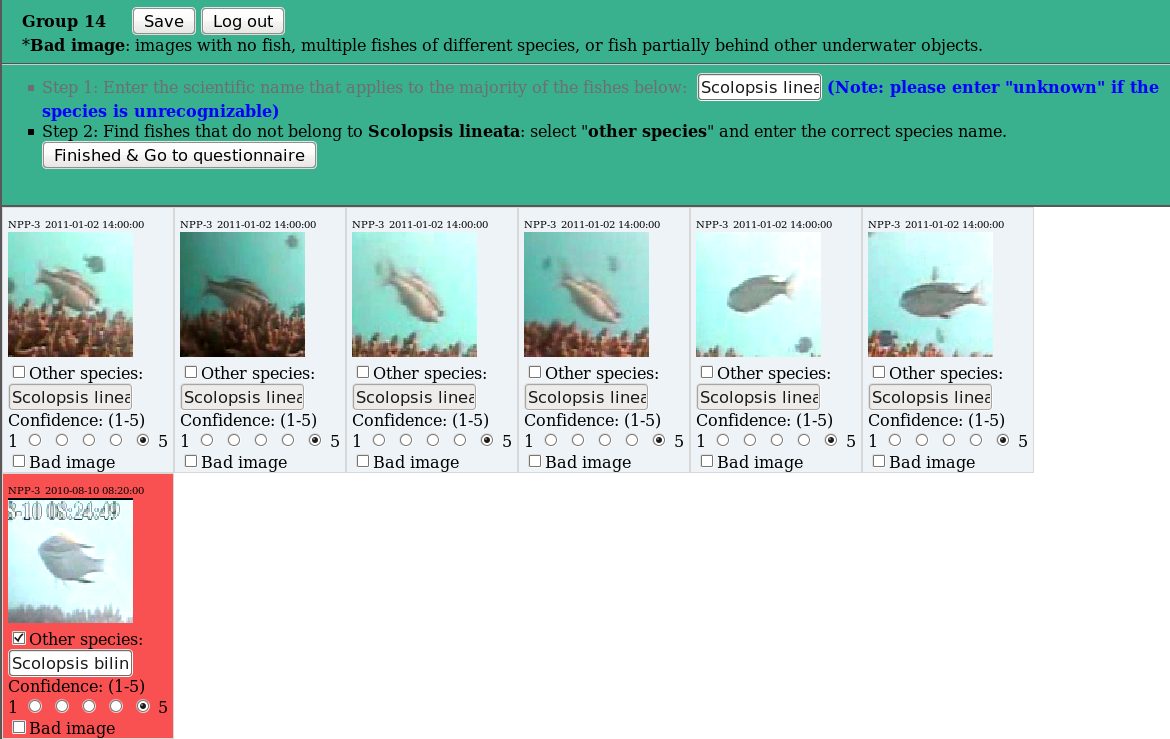
\includegraphics[width=0.48\textwidth, height=0.25\textwidth]{expertlabel.png}
\label{fig:expert_interface}
}
\subfigure[Game interface for non-experts]{
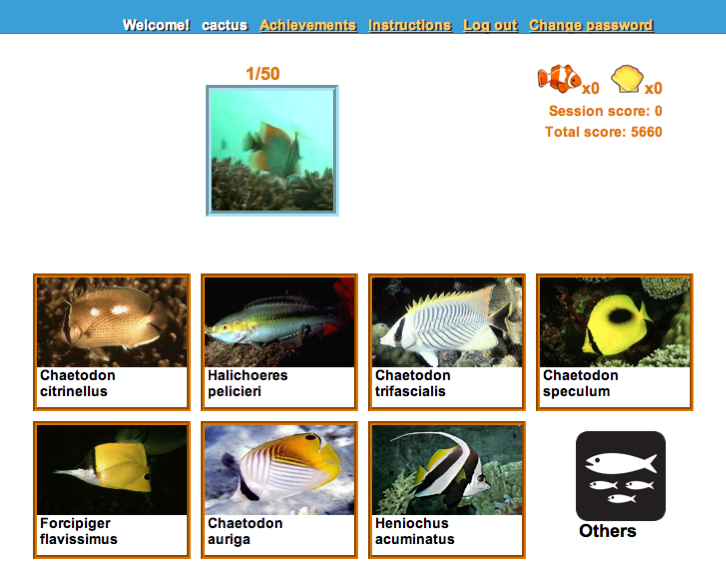
\includegraphics[width=0.45\textwidth, height=0.25\textwidth]{nonexpert_interface.png}
\label{fig:nonexpert_interface}
}
%\miniskip
\caption{Expert and game interfaces for labeling fish species.}
\end{figure*}

%==============OLD =======================================
\if 0
As already mentioned, experts are expensive and a scarce resource.
Therefore we ask our experts to label only a small subset of our data
and developed a cluster-based interface to facilitate their labeling
process. The images labeled by the experts are used as gold standard
for the evaluation of non-expert labels.

%\miniskip
\subsection{Experiment setup}
%
Two students manually clustered 3000 images randomly chosen from our
video data. The students were allowed to discuss and in total obtained
28 clusters. We present the images to the experts in a labeling
interface as shown in Figure~\ref{fig:expert_interface}. 
%
Using this interface, the expert first enters the species name that
applies to the majority of the images in a cluster. 
%in the top-right text box. 
Once the name is entered, all images within the cluster are
automatically assigned with the same species name. Then, the expert is
asked to select those images that should not belong to that cluster.
By selecting these images, he/she can also input the correct species
names for them. 
%for them in the text box under each image. 
In this manner, in the worst case, the expert will have to manually
assign a species name to each of the images, i.e., when the clustering
is so bad that each image within a cluster represents a different fish
species. In the best case, i.e., when the cluster is pure, the expert
only needs to enter the species name once.
%
After finishing annotation, we submit the expert to a questionnaire in
order to collect information such as whether the labeling task was
difficult for him/her, and why it was difficult. 
%
To limit the amount of effort experts need to examine the clusters, at
most 30 images are randomly selected from each cluster and shown to
the experts. As the size of the clusters is unevenly distributed,
e.g., only some of the clusters contain more than 30 images, we obtain
a total of 190 labeled images.

Since we collect experts' labels to create a gold standard, we need
experts to assign labels to the best of their ability. To this end we
put no constraints on the amount of time experts spent on the labeling
task or on the use of additional resources. In general experts were
able to recognize a fish based on their knowledge. For ``difficult"
species, they consulted textbooks to verify their judgement.  

\subsection{Data obtained}
%\label{subsec:exp_data}
We invited 3 marine biologists (referred to as E1, E2 and E3) to
participate in the expert labeling task. They have research experience
of 30, 10 and 25 years in Taiwanse coral reef fish, respectively. 
  
An analysis of the labels assigned by the experts to the 190 fish
images reveals that the biologists do not always agree on the species
names for an image.
%For 82.6\% of the images, at least two biologists agreed on a species
%name; for 56.3\% of the images, all biologists agreed on a name
%(including the cases where two biologists agreed on a species name
%while the third biologist indicated that he/she cannot identify the
%fish).
We use Cohen's kappa~\cite{Cohen60} to measure the agreement between
the expert labels, assuming the complete category set consists of all
unique species mentioned in the labels provided by the experts. 
%See Table~\ref{tab:expert_agree}.
\begin{table}[h!]
%\vspace*{-\baselineskip}
\centering
 \begin{tabular}{@{~}l@{~~~}l@{~~~}l@{~~~~~}l@{~~~}l@{~}}
 \hline
  & \multicolumn{2}{l}{Species level} & \multicolumn{2}{l}{Family level}\\
  Comparison & Avg.$\kappa$ & Sdv. & Avg.$\kappa$ & Stv.\\
  \hline
  E1 vs. E2  & 0.55 & 0.008 & 0.85 & 0.004\\
  E1 vs. E3  & 0.48 & 0.008 & 0.75 & 0.000\\
  E2 vs. E3  & 0.67 & 0.006 & 0.76 & 0.0001\\
  \hline
 \end{tabular}
  \caption{Cohen's kappa for measuring expert agreement.}
\label{tab:expert_agree}
%\vspace*{-\baselineskip}
\end{table}
%

In addition, we find that sometimes the biologists are not sure which
species a fish should belong to: 1) one of the experts assign labels
such as ``A or B'' to 3 images, and 2) in 45 cases (each case is a
pair of image and expert, in total we have 190 x 3 cases) a family or
higher level label is assigned. 
%39 genus
%For images with genus level labels there are no case where all 3 experts agree on a label.  
In the former case, we consider both labels mentioned, and in the
latter case, we consider all species under a higher level label as
possible target labels.  Thus it is possible that an image has
multiple labels assigned by a single expert.  In total, 288 species
and 20 families were mentioned as labels for the 190 images. 
%
Since Cohen's kappa does not handle multiple labels of a single rater,
we handle this situation as follows.\footnote{Notice that here we could
use other measures such as Fleiss' kappa to compute the agreement
between multiple raters. However we chose to use pairwise Cohen's
kappa for the following reason. In later experiment, we will compare
the agreement between aggregated non-expert labels and the expert
labels, to the agreement among the expert labels. In that case, we
will be comparing the agreement among 4 raters (3 experts and the
aggregated non-expert), to the agreement among 3 raters (3 experts).
The values of Fleiss' kappa calculated with different number of raters
are not comparable.} 
%First, we evaluate the agreement between labels at both species and family levels:
%it is expected that at family level, cases with such situation will be greatly reduced. 
%Second, 
When there exist multiple labels for an image assigned by one expert,
we randomly draw one of them as the target label being evaluated; we
repeat this process 100 times and report the averaged $\kappa$ and its
standard deviation over the 100 runs\footnote{Notice that the
agreement calculated in this way is rather conservative}. We evaluate
labels at both species and family level.

%
\begin{figure*}[t!]
\centering
\subfigure[Species recognition interface for experts]{
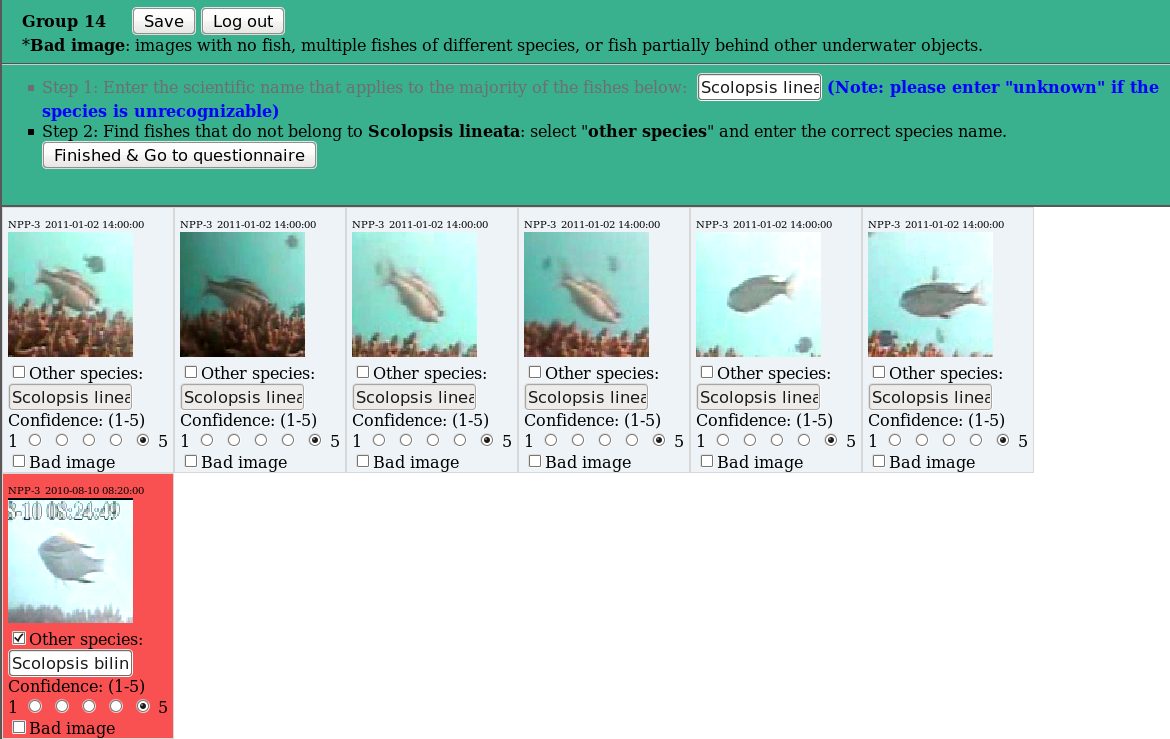
\includegraphics[width=0.48\textwidth, height=0.25\textwidth]{expertlabel.png}
\label{fig:expert_interface}
}
\subfigure[Game interface for non-experts]{
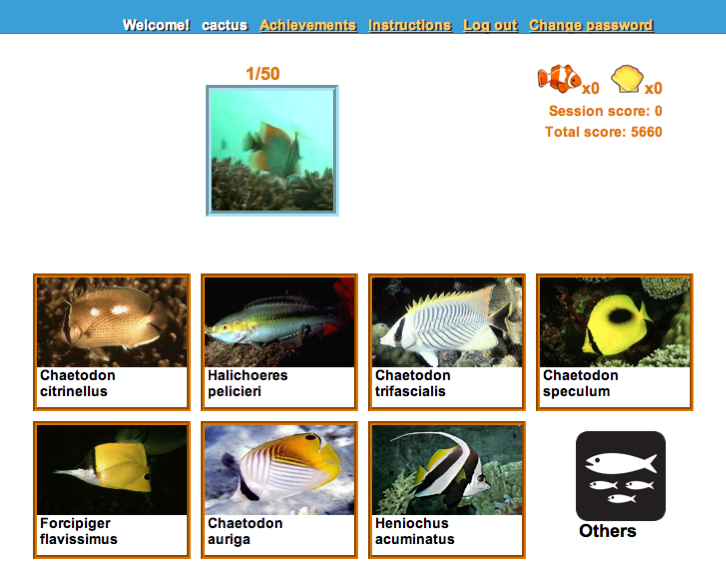
\includegraphics[width=0.45\textwidth, height=0.25\textwidth]{nonexpert_interface.png}
\label{fig:nonexpert_interface}
}
\caption{Expert and game interfaces for labeling fish species.}
\end{figure*}

Results in Table~\ref{tab:expert_agree} show that at the species
level, the agreement between experts is only moderate, while at family
level, a much stronger agreement can be found, but still not perfect.
This result suggests that our labeling task is not trivial even for
experts. 
%
Further, from the questionnaire we learn that according to the
experts, the top factors that make recognition difficult are: 1)~the
low quality of the images; and 2)~the fact that some species are
visually very similar and not distinguishable using the features that
can be observed from the images.  For example, the main feature
biologists use to distinguish Chromis Chrysura and Chromis
Margaritifer is their body size, while in video footage the size of a
fish depends on its distance to the camera, and therefore it does not
provide enough information. 
%

Note that we treat experts' labels as the ground truth. That is, if
two experts disagree, it does not mean that they make mistakes, but
that these species are not distinguishable given available
information.  The purpose of measuring the agreement between experts
is to provide a sanity check, or a (loose) upper bound for the
performance of the fish labeling task. 

\fi

